\chapter{Approccio proposto}
\label{chap:approccio}
\vspace{1cm}
Nel Capitolo \ref{chap:SOA} sono state descritte alcune soluzioni proposte 
relative al lavoro oggetto di questa tesi, in particolare algoritmi esatti ed
euristici di ottimizzazione basati su varie tecniche.
% TODO & FIXME aggiungere qualcosa (tipo pro/contro)

In questo capitolo verrà descritto l'approccio utilizzato per risolvere il 
problema di scheduling dei task tenendo in considerazione le comunicazioni e 
riconfigurazioni introdotte.

Il capitolo è organizzato secondo la seguente struttura: nella Sezione 
\ref{sec:integrazioneToolchainFASTER} viene descritta l'integrazione 
dell'algoritmo di scheduling con il componente che gestisce il mapping dei task, 
con accenni alle interfacce esterne che collegano il componente 
agli altri strumenti utilizzati nella toolchain di \acs{FASTER}; la Sezione 
\ref{sec:panoramicaMetodologia} descrive  ad alto 
livello il funzionamento dell'algoritmo di scheduling, fornendo una 
panoramica delle fasi in cui questo si divide; la Sezione 
\ref{sec:euristicaSceltaTask} contiene una descrizione dettagliata della fase 
più delicata del procedimento di scheduling, la scelta del task migliore da 
considerare ad ogni passo di decisione; la Sezione 
\ref{sec:osservazioniConclusive} fornisce un riepilogo dei concetti importanti 
presentati in questo capitolo.


\section{Integrazione nella toolchain di \ac{FASTER}}
\label{sec:integrazioneToolchainFASTER}

Come descritto nel precedente capitolo, l'obiettivo del progetto europeo 
\ac{FASTER} è fornire un framework per la sintesi ad alto livello di 
applicazioni, scritte in linguaggio di programmazione C, su vari dispositivi 
riconfigurabili; la toolchain che permette di realizzare questa sintesi è 
composta da varie fasi eseguite in sequenza. Ogni fase deve essere il più 
possibile self-contained, ovvero deve poter essere invocata separatamente e non 
deve avere nozioni sul funzionamento interno delle altre fasi.

Condizione necessaria perchè ciò accada è la definizione di specifiche 
interfacce per ogni strumento che deve essere invocato. Ad esempio, la fase di 
mapping ha la propria interfaccia di input e di output; lo scheduler 
(incapsulato nell'algoritmo evolvibile di esplorazione delle soluzioni di 
mapping) ha anch'esso una interfaccia di input e una di output, contenenti tutte 
le strutture dati necessarie per l'elaborazione e per la memorizzazione delle 
informazioni calcolate dall'algoritmo, rispettivamente. 

\begin{figure}
 \begin{center}
  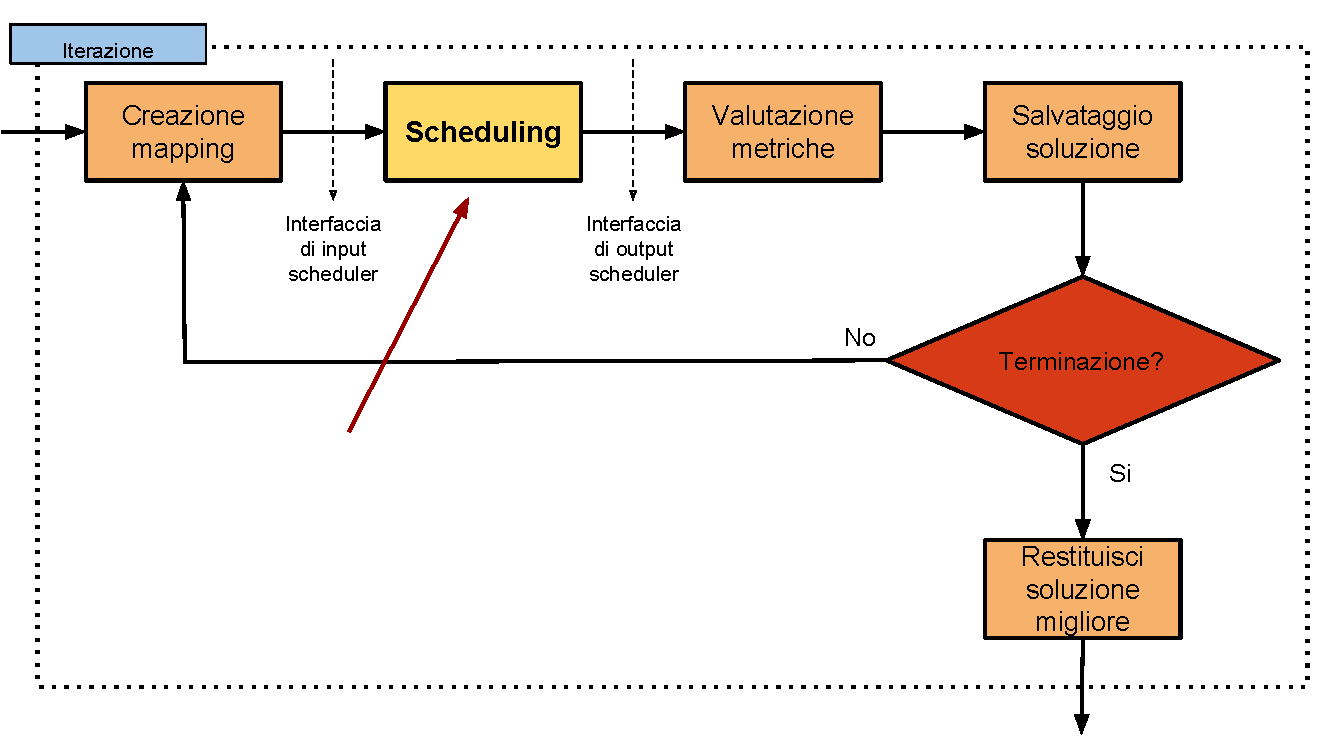
\includegraphics[width=0.9\textwidth]{capitoli/figure/cap3/MapperWorkflow.pdf}
  \caption{Flusso di lavoro dell'algoritmo di esplorazione.}
  \label{fig:mapperWorkflow}
 \end{center}
\end{figure}

A livello dell'algoritmo di mapping, dunque, si avrà un flusso di lavoro come 
rappresentato nella Figura \ref{fig:mapperWorkflow}, in cui è messo in evidenza 
dove si colloca la fase di scheduling oggetto del lavoro rispetto al flusso 
dell'algoritmo di esplorazione, con le relative interfacce di input e output.


\section{Panoramica della metodologia}
\label{sec:panoramicaMetodologia}


\section{Euristica di scelta dei task}
\label{sec:euristicaSceltaTask}


\section{Osservazioni conclusive}
\label{sec:osservazioniConclusive}
